\documentclass{article}
\usepackage[left=3cm, right=3cm, top=3cm, bottom=3cm]{geometry}
\usepackage{graphicx} 
\usepackage{amssymb}
\usepackage{amsthm}
\usepackage{amsmath}
\usepackage{amsbsy}
\usepackage{bm}
\usepackage{hyperref}
% anything surronded by this new command will not do anything
\newcommand{\mycomment}[1]{} 
% Use like: \halfopen{0}{1} to get (0,1] 
\newcommand\halfclosed[2]{\ensuremath{[#1,#2)}}
\newcommand\halfopen[2]{\ensuremath{(#1,#2]}}
\newcommand{\C}{\mathbb{C}}
\newcommand{\R}{\mathbb{R}}
\newcommand{\Z}{\mathbb{Z}}
\newcommand{\N}{\mathbb{N}}
\newcommand{\Q}{\mathbb{Q}}
\renewcommand{\P}{\mathbb{P}}
\setlength\parindent{0pt}


\title{KAN Reference Page}
\author{Nash Rickert}

\begin{document}
\maketitle

\section{Overview}
According to the original paper, in a KAN, ``every weight parameter is replaced by a [learnable] univariate function parametrized as a spline'', replacing the linear weights of a traditional MLP. Thus it is important to understand what this actually means in order to properly understand and communicate about the model.

\section{Definitions and Terms}

\subsection{B-Splines, Mathematically}
According to wikipeida, ``a spline is a function defined piecewise by polynomials''. Constrastingly, ``a B-spline (short for basis spline) is a type of spline function designed to have minimal support (overlap) for a given degree, smoothness, and set of breakpoints (knots that partition its domain)''. Note that the 'B' in 'B-spline' has nothing to do with the degree or smoothness of the B-spline. A B-spline of order $n$ is a piecewise polynomial of degrees $n - 1$. The points where these polynomials meet are called knots. Notably, ``Any spline function of a specific degree can be uniquely expressed as a linear combination of B-splines of that degree over the same knots''. Thus problems involving splines largely reduce to considering B-splines, which is probably why the paper tends to use the terms interchangably.\\\\
Wikipedia states that B-splines are continuous at their knots and if the knots are distinct, they are continuous up to the derivative of degree $n - 2$ where the B-spline is of order $n$. Each coincident knot reduces the continuity of degree order by $1$ (I believe in our ML context, knots would never be coincident. It is at least never mentioned in the paper).

\subsection{B-Splines, In the Paper}
The model parameterizes the univariate activation functions as a B-spline. As far as I can tell, the paper uses the term 'spline' and 'B-spline' interchangably, although they are actually mathematically distinct. Importantly, the model does not actually learn the B-spline parameterization directly, but instead learns to adjust the weights of local B-spline basis functions (the terminology is confusing here). If $f(x)$ is our learned B-spline, then $f(x) = \sum_{i} c_i \cdot B_i(x)$ where $B_i(x)$ are fixed induvidual B-spline basis functions and $c_i$ are the learned coefficients. The $B_i$ are generally only supported over a small interval comprising several knots (such as degree + 2 knots). They join with the continuity requirements discussed in the previous section. The basis function itself is entirely determined by the hyperparameters of degree and knot count/position. For example, a degree $2$ B-spline basis function would be
\begin{itemize}
\item Zero everywhere but over 3 consecutive knot intervals
\item Consisting of one quadratic polynomial piece within each interval
\item The pieces connect with $C^1$ continuity at the knots
\end{itemize}
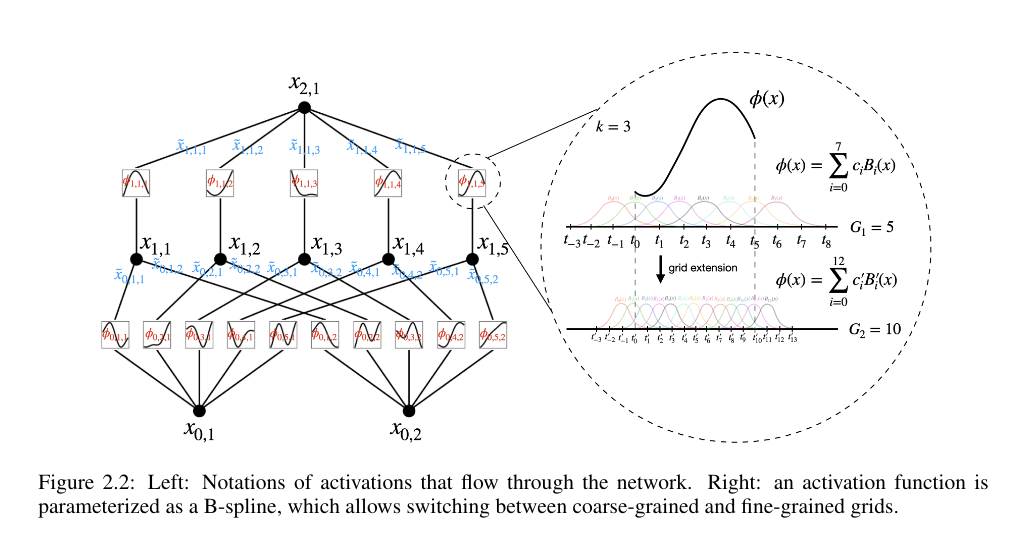
\includegraphics[scale = 0.5]{figure1.png}


\subsection{Other Details}
Each edge actually also contains a basis function, not just the spline. This graphic should make that relatively clear:\\
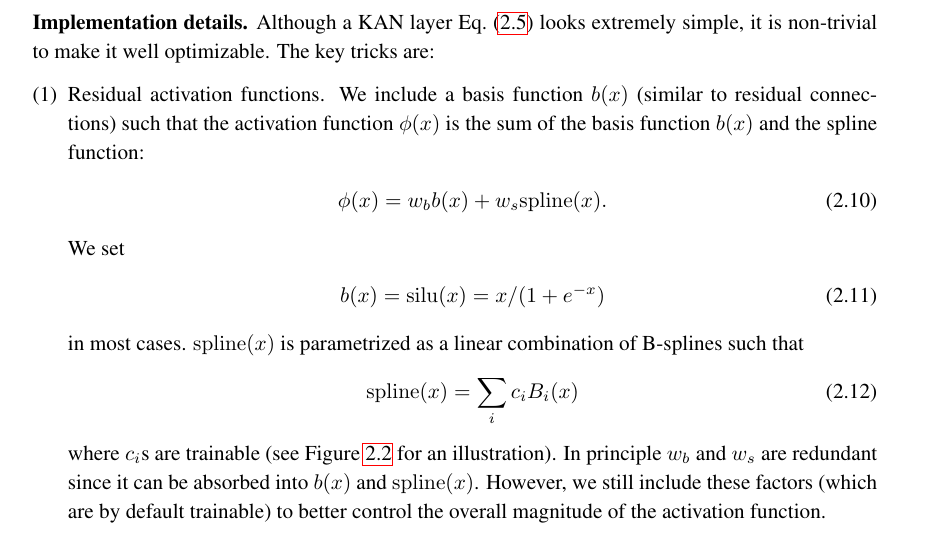
\includegraphics[scale=0.5]{figure2.png}\\
My understanding is that, at least by default, knots are uniformly spaced throughout the domain. It might be the case that this can be adjusted so knots are placed adaptively such that training data is roughly equally spaced within intervals. I do not believe that the authors implemented it so that knots positions can be learned. As a final note, some other implementation use different functions other than B-splines, which appear promising and potentially faster (though probably immaterial for us if we use lookup tables).

\subsection{C Implementation}
As mentioned above, in order to properly benchmark a KAN, I will make a general C implementation that utilizes lookup tables to approximate the values of the splines at points in the domain. To do this, I will make a struct which stores the lookup values in an array alongside meta data of the xmin and xmax values which correspond to the first and last entries of the table. A lookup function will accept an x value as input and interpolate between the two nearest indexes of the lookup table to find an appropriate approximation of the function, returning that value. Since our desired KAN architecture is currently unknown and we wish to benchmark and integrate across a broad range of possible designs, I will seek to make the implementation as general as possible. The actual details of the KAN approximation, regarding B-splines or other methods, will be abstracted into the lookup table as the symbolic approximations are not really important for our hardware implementation. Ideally, the only part of the implementation that would remain 'ungeneral' would be the specific parsing and transfer of model parameters from python to C, which would require particular filenames and knowledge of the KAN implementation and parameters to properly implement.

\subsection{References}
\url{https://pages.mtu.edu/~shene/COURSES/cs3621/NOTES/spline/B-spline/bspline-basis.html}\\
\url{https://en.wikipedia.org/wiki/B-spline}\\
\url{https://en.wikipedia.org/wiki/Spline_(mathematics)}\\
\url{https://arxiv.org/pdf/2404.19756}

\end{document}
